% \documentclass[14pt]{extarticle}
\documentclass[bibliography=totocnumbered]{scrartcl}
% \usepackage[english]{babel}
\usepackage[russian]{babel}
\usepackage[utf8x]{inputenc}
\usepackage{amsmath}
\usepackage{graphicx}
\usepackage[colorinlistoftodos]{todonotes}
\usepackage{amssymb}
\usepackage{amsmath}
\usepackage{graphicx}
\usepackage[margin=.8in]{geometry}
\usepackage{listings}
\usepackage[section]{placeins}
\usepackage{listings}
\begin{document}

\begin{titlepage}
\newgeometry{margin=2cm}
\newcommand{\HRule}{\rule{\linewidth}{0.5mm}}
\center
\textsc {
\footnotesize{
минобрнауки россии\\
федеральное государственное бюджетное образовательное учреждение\\
высшего профессионального образования}\\
\large{Воронежский государственный университет}
}\\[1.0cm]
\textsc{\largeФакультет компьютерных наук}\\
\textsc{\footnotesizeКафедра информационных технологий}\\[1.0cm] 
\textsc{\Large Эссе}\\[0.5cm]
\HRule \\[0.4cm]
{ \huge \bfseries Системная инженерия на примере системы «Газовый котёл»}\\[0.4cm] % Title of your document
\HRule \\[1.5cm]


\begin{flushleft} \large
% \emph{Зав. кафедрой:} Э.К. \textsc{Алгазинов}, д. ф-м н., проф.\\
\emph{Студент:} А.А. \textsc{Валиков} \\
% \emph{Руководитель:} А.В. \textsc{Стромов}, к. ф-м н. % Supervisor's Name
\end{flushleft}

\vfill
\begin{center}
Воронеж 2018
\end{center}
\end{titlepage}

\tableofcontents

\newpage

\section{Введение}

\subsection{Функциональные требования стейкхолдеров}

\paragraph{Пользователи}
\begin{itemize}
  \item Низкие расходы (цена котла, потребление газа, обслуживание)
\end{itemize}

\paragraph{Газовая служба}
\begin{itemize}
  \item Безопасность (например, газовый затвор имеет дублированную схему)
\end{itemize}

\paragraph{Производитель}
\begin{itemize}
  \item Высокий спрос
  \item Минимальные затраты на ресурсы и рабочую силу
\end{itemize}
Основная функция -- \textbf{нагревать воду и перемещать её по системе отопления}

\subsection{Конструкционные ограничения архитектуры}
Котёл представляет из себя сложную систему, опишем его в общем, с некоторыми допущениями.

\begin{figure}[htp]
  \centering
  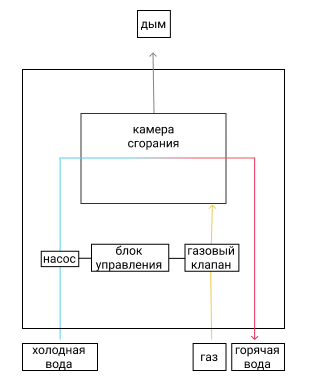
\includegraphics[scale=1.00]{arch.png}
\end{figure}

\subsection{Описываемая система как холон в иерархии}
\subsection{Системы: целевая, обеспечивающая, в эксплуатационной среде}

\section{Жизненный цикл системы согласно V-диаграмме}
\subsection{Определение требований}
\subsection{Архитектурное проектирование}
\subsection{Рабочее проектирование}
\subsection{Изготовление}
\subsection{Интеграция}
\subsection{Приём в эксплуатацию и эксплуатация}

\section{Практики системной инженерии}

\subsection{Сбор требований}
\subsection{Анализ требований}
\subsection{Архитектурный дизайн}
\subsection{Изготовление}
\subsection{Интеграция}
\subsection{Проверка всей системы}
\subsection{Переход к эксплуатации}
\subsection{Валидация}
\subsection{Эксплуатация}
\subsection{Обслуживание}
\subsection{Вывод из эксплуатации}
\end{document}